\section{Additional numerical and empirical results}
\label{sec:supp-numerics}

All results in this section were generated with the implementation version
recorded in the result registry. The registry contains 95 point/risk
simulation objects, 24 multiplier-band objects, 115 AI downstream objects, 6 AI
band objects, and two application objects (242 objects total), each with an exact
path and SHA-256 hash.

\subsection{Simulation inventory}

The simulation manifest contains 119 configurations spanning oracle
mechanisms, a five-cell vanishing-curvature path, estimated regression paths,
selective verification, scarce-reference scaling, nuisance and distributional
perturbations, multiplier bands, estimated propensities, discrete outcomes,
and two-dimensional localization. Every replication uses the same generated
data, verification mask, fold assignment, and threshold grid across methods.
Primary modules use 2,000 replications, secondary modules use 1,000, and
two-dimensional modules use 500. The multiplier-band module uses 4,999
Rademacher draws per replication. L'Ecuyer--CMRG streams assign deterministic,
scenario-specific data streams. Multiplier seeds are deterministic functions
of replication and method, are recorded in every object, and are shared across
band scenarios to provide common multiplier draws.

\subsection{Threshold-level CDF evaluation}

The scalar result objects retain ISE, tail loss, quantile loss, borrowing,
and coverage summaries but not every threshold-level estimate. Before producing
the new curves, we selected three existing settings to represent aligned
borrowing under 10\% random verification, a moderate surrogate under 5\%
selective verification, and local reversal under 10\% random verification.
The choice was based on these scientific roles rather than the appearance of
the curves. Each setting was recomputed over its first 500 deterministic
random-number streams without changing its data-generating
mechanism, learner, bandwidth, folds, or threshold grid. The artifact stores
the truth, mean and median rearranged CDF, pointwise bias, pointwise RMSE,
central estimate quantiles, the first-stream diagnostic bands, all seeds, and
source hashes. All twelve integrity checks pass.

The application panels use the first reference sample at the following targets:
50\% relative humidity for EPA, 75 minutes for VitalDB, and 10\% random review
at \(x_0=0\) for the AI study. The EPA and AI Adaptive bands contain their
complete-data or population benchmarks. The VitalDB band does not, and
its fixed-mask ISE ordering differs from the repeated-mask mean ordering. These
panels remain diagnostic examples rather than empirical coverage estimates.

\begin{figure}[H]
\centering
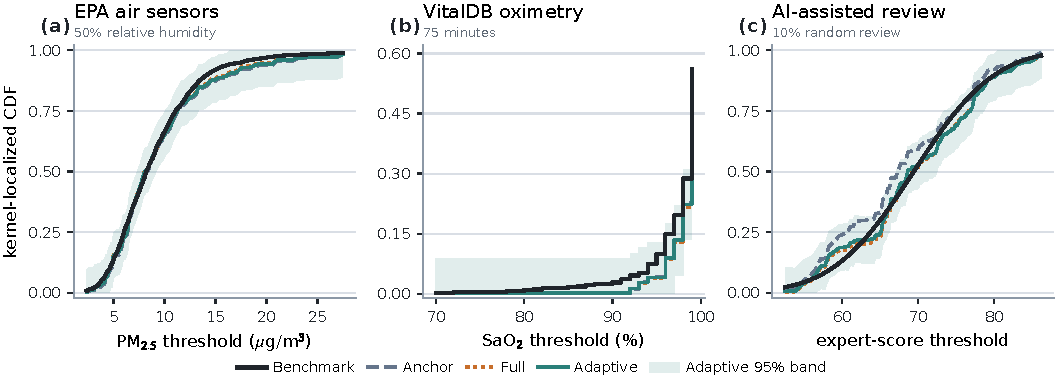
\includegraphics[width=\textwidth]{../paper/figures/figure4_application_evidence.pdf}
\caption{Conditional-CDF estimates from one fixed reference sample in each
study. Each panel uses a 10\% random-reference sample at a target fixed before
the curves were produced. Black denotes \(F_{h,\mathrm{emp}}\) for EPA and
VitalDB and the frozen \(F_{h,0}\) for the AI benchmark; slate dashed, orange
dotted, and teal solid curves denote Anchor, Full, and Adaptive. The teal
ribbon is the Adaptive 95\% simultaneous band. The EPA and AI bands contain
their benchmarks; the VitalDB band does not.}
\label{fig:supp-fixed-application-cdfs}
\end{figure}

\subsection{Oracle mechanisms}

Supplementary Table~\ref{tab:sim-oracle} reports the oracle geometry. The sign
of $2G_h-H_h$ matches the realized anchor-minus-Full ISE direction in all 18
cells. M4 now has separate clipped and raw paths. The clipped paths have
positive transfer signals, while the raw paths have negative signals; both
versions agree with their realized risk directions. M5--M6 have
$\lambda_h^{\mathrm{or}}=0$, mean estimated coefficients below $10^{-4}$, and harmful
full borrowing.

Oracle $m_0(X,S)$ reduces mean ISE relative to the $X$-anchor by 25.3--28.0\%
in M1--M2. In M2, the conservative candidate improves on the anchor but does
not attain the oracle-$m$ risk, illustrating the positive-semidefinite
augmentation excess directly.

\subsection{Candidate regression methods and local failure}

Supplementary Table~\ref{tab:sim-feasible} compares the primary
location--scale learner with misspecified parametric and nearest-neighbor
candidates. At moderate surrogate noise, Adaptive gains are 23.7\%, 25.3\%,
and 22.4\% for the primary, L2, and L3 learners. Across the strong-to-weak
surrogate sequence, primary gains decline from 48.5\% to 7.6\%; the analogous
L2 range is 49.8--11.0\% and the L3 range is 37.0--8.0\%.

The local-reversal scenario N5 is the main failure audit. Adaptive reduces
mean borrowing to 0.0017 and negative-transfer frequency to 1.5\%, compared
with 82.3\% for Full. Its mean ISE remains 0.066\% above the anchor because a
small number of loss realizations dominate the paired mean. This result
shows that Adaptive greatly reduces the risk increase caused by local reversal,
but does not establish uniform or finite-sample dominance.

\subsection{Distributional perturbations and localization dimension}

Adaptive gains are 15.6\%, 17.8\%, and 24.7\% under standardized $t_3$,
standardized $\chi^2_3$, and Gaussian-mixture errors, compared with 22.0\%
under Gaussian errors. For the ten-level outcome, category-scale oracle truth
produces a 22.5\% Adaptive gain and a 25.9\% Full gain. The old apparent loss
was caused by evaluating discrete outcomes against a continuous-scale truth
engine.

With $X=(X_1,X_2)$, a product Epanechnikov kernel, and $h=M^{-1/6}$, Adaptive
gains range from 20.9\% to 24.4\% over
$M\in\{2{,}000,5{,}000\}$ and $p_M\in\{0.10,0.20\}$.

\subsection{Bandwidth, curvature, and estimated propensities}

The bandwidth and denominator-floor checks preserve the primary risk ordering.
The numerical analyses use a denominator floor of $10^{-8}$.
We vary the candidate-path scale over
$s\in\{1,0.5,0.25,0.125,0\}$, so normalized curvature follows $s^2$,
the effective correction decreases from 0.899 to zero, and
Adaptive-minus-path-oracle regret decreases from $6.01\times10^{-5}$ to zero.

Eight exploratory configurations estimate verification probabilities on the
fitting fold. Adaptive gains range from 22.9--45.4\%, while mean borrowing
ranges from 0.408 to 0.600. These results demonstrate sensitivity of the
selected path to propensity estimation; inferential validity still requires
the local product-rate condition in Section~\ref{sec:supp-pi-adaptive}.

\subsection{Scarcity and multiplier bands}

Supplementary Table~\ref{tab:sim-scarcity} reports scaling over four sample
sizes and four reference fractions. For $Mp_Mh\geq30$, scaled ISE lies in
0.319--0.358 for the anchor and 0.241--0.286 for Adaptive. The rescaling is
stable over the grid, while selective placement changes the covariance
constant at the same nominal reference fraction.

Supplementary Table~\ref{tab:sim-bands} reports the 24 multiplier cells.
At the lowest nominal rate index, the selective-verification cells give
Adaptive coverage 0.910--0.935 and anchor coverage 0.908--0.932. The minimum
Adaptive estimate has Monte Carlo standard error 0.0090 and a 95\% Wilson
interval of 0.8907--0.9262. Adaptive coverage over all cells ranges from 0.910
to 0.953. Mean coverage under selective verification increases from 0.9220 at
$p_M=0.05$ to 0.9435 at $p_M=0.20$.
Aligned surrogates reduce
integrated width to 0.760--0.981 of the anchor width; locally reversed paths
produce ratios within 1.000--1.003, eliminating nearly all width gain.
The minimum role-fold verified support averages about five in the lowest
selective cells. Table~\ref{tab:band-local-information} shows pooled raw
coverage of 0.911 for counts 4--5 and 0.945 for counts of at least 10.

A pre-specified seven-cell sensitivity used the same data streams and 4,999
multiplier draws. Increasing rearrangement of the endpoints raised coverage in
several low-information cells but did not restore the nominal level uniformly.
A pointwise-studentized supremum band produced coverage 0.358--0.633 and was
13--24\% narrower than the unstudentized band. It failed the selection rule, so
the raw-process band remains primary.

\subsection{Application configurations}

The EPA analysis uses
\(X=(\mathrm{RH}-50)/20\),
\(S=\log(1+\mathrm{PurpleAir})\), and
\(Y=\log(1+\mathrm{reference\ PM}_{2.5})\). Targets
\(x_0\in\{-1,0,1\}\) correspond to 30\%, 50\%, and 70\% relative humidity;
the Epanechnikov bandwidth is \(h=0.5\), and the 101 thresholds span the
empirical 0.01--0.99 quantiles of transformed \(Y\).

The VitalDB analysis uses
\(X=\log(1+\mathrm{elapsed\ minutes})\), \(S=\mathrm{SpO}_2\), and
\(Y=\mathrm{SaO}_2\). Targets are 30, 75, and 180 minutes, the Epanechnikov
bandwidth is \(h=0.55\), and the threshold grid is \(70{:}99\).

The AI analysis uses standardized complexity \(X\), automated score \(S\),
and the mean of three expert ratings as \(Y\), with \(x_0=0\), \(h=0.3\),
and 101 thresholds defined by point-target conditional quantile levels
0.02--0.98. For confidence-triggered designs, the broadly observed vector is
\(W=(X,S,C)\), where model confidence \(C\) enters the known verification
probability; the augmentation candidates use \((X,S)\). The risk benchmark is
the frozen population \(F_{h,0}\).

\subsection{EPA details}

The EPA source archive is verified by SHA-256 before extraction. The
uncorrected PurpleAir records are aggregated to 2,814 site-days, and calendar
weeks are assigned to regression fitting, weight selection, and CDF evaluation.
At the 10\% random budget, Adaptive gains
are 52.2--60.3\%, with paired intervals excluding zero. A single weekly
cluster-multiplier diagnostic gives 19--30\% narrower Adaptive bands and
complete-data containment at all three humidity targets; it is not a
repeated-coverage result.

\subsection{VitalDB details}

The VitalDB acquisition and hash-selection rules produce 8,476 eligible pairs
and 3,178 subject-level observations. At the 10\% random budget, Adaptive gains
are 11.8\%, 11.2\%, and 2.95\%. Within-grid information multipliers are 1.109,
1.102, and 1.027 at 30, 75, and 180 minutes. Full has lower mean ISE, but its
paired advantage is conclusive only at 30 minutes. Adaptive reduces observed
negative-transfer frequency relative to Full at all targets; the paired
interval excludes zero at 75 and 180 minutes.

\subsection{AI-assisted evaluation details}

The corrected reference uses fixed expert biases $(-1,0,1)$ while retaining
the same dossier text and 5,997 valid model responses. On Corpus A, bias,
MAE, and RMSE are 0.350, 2.415, and 3.058; Pearson and Spearman correlations
are 0.946 and 0.942.

The primary evaluator is \texttt{deepseek-v4-pro};
\texttt{deepseek-v4-flash} is used for the model-sensitivity analysis. Both use
the frozen dossier text and rubric. A canonical call manifest links each
corpus row to its request hash and cached response-file checksum; the model
outputs themselves were fixed before any reference mask was drawn. A companion
cache manifest checksums all retained primary and sensitivity responses.

Under random review, Adaptive gains are 53.9--59.9\%. For fractions up to 0.10,
the anchor needs 2.28--2.50 times the actual fraction to match Adaptive risk
within the evaluated grid. Under local under-review and local reversal,
Adaptive borrowing collapses toward zero and limits mean loss to at most
0.39\%, whereas Full remains harmful. Representative AI multiplier cells have
Adaptive coverage 0.940--0.974 and narrower bands than the anchor.

\subsection{Complete simulation tables}

\begin{table}[p]
\centering
\caption{Oracle mechanism results. The realized gain is anchor ISE minus full-borrowing ISE.}
\label{tab:sim-oracle}
\begin{tabular}{lcccccc}
\toprule
Scenario & $G_h$ & $H_h$ & $2G_h-H_h$ & $\lambda_h^{\mathrm{or}}$ & $E(\widehat\lambda_h)$ & Realized gain \\
\midrule
M1-R1 & 0.575 & 0.575 & 0.575 & 1.000 & 0.900 & 0.001 \\
M1-R2 & 0.861 & 0.861 & 0.861 & 1.000 & 0.852 & 0.001 \\
M2-R1 & 0.287 & 0.144 & 0.431 & 1.000 & 0.998 & 0.001 \\
M2-R2 & 0.431 & 0.215 & 0.646 & 1.000 & 0.984 & 0.001 \\
M3-R1 & 0.750 & 0.998 & 0.501 & 0.751 & 0.734 & 0.001 \\
M3-R2 & 1.131 & 1.515 & 0.746 & 0.746 & 0.721 & 0.001 \\
M4-R1 & 0.867 & 1.445 & 0.290 & 0.600 & 0.595 & 0.001 \\
M4-R1-unclip & 1.437 & 3.593 & -0.719 & 0.400 & 0.399 & -0.001 \\
M4-R2 & 1.321 & 2.239 & 0.403 & 0.590 & 0.582 & 0.001 \\
M4-R2-unclip & 2.153 & 5.381 & -1.076 & 0.400 & 0.391 & -0.002 \\
M5-R1 & -0.269 & 0.130 & -0.667 & 0.000 & 0.000 & -0.001 \\
M5-R2 & -0.404 & 0.196 & -1.005 & 0.000 & 0.000 & -0.002 \\
M6-R1 & -0.269 & 0.130 & -0.667 & 0.000 & 0.000 & -0.001 \\
M6-R2 & -0.404 & 0.196 & -1.005 & 0.000 & 0.000 & -0.002 \\
M7-R1 & 0.507 & 0.532 & 0.481 & 0.952 & 0.873 & 0.001 \\
M7-R2 & 0.733 & 0.779 & 0.687 & 0.941 & 0.837 & 0.001 \\
M8-R1 & 0.567 & 0.687 & 0.448 & 0.826 & 0.794 & 0.001 \\
M8-R2 & 0.836 & 1.025 & 0.646 & 0.815 & 0.742 & 0.001 \\
\bottomrule
\end{tabular}
\end{table}

\begin{table}[p]
\centering
\caption{Feasible estimator results. Relative gain is the percentage reduction in mean ISE from the X-anchor.}
\label{tab:sim-feasible}
\resizebox{\textwidth}{!}{%
\begin{tabular}{lccccccc}
\toprule
Scenario & ISE anchor & ISE Adaptive & ISE Full & Rel. gain & $\widehat\lambda_h$ & NT Adaptive & NT Full \\
\midrule
F1-p0.05 & 0.0099 & 0.0075 & 0.0069 & 23.4 & 0.693 & 0.332 & 0.346 \\
F1-p0.10 & 0.0048 & 0.0036 & 0.0035 & 24.0 & 0.784 & 0.339 & 0.360 \\
F1-p0.20 & 0.0024 & 0.0019 & 0.0018 & 21.5 & 0.850 & 0.362 & 0.383 \\
F2-L2-t16 & 0.0049 & 0.0044 & 0.0043 & 11.0 & 0.699 & 0.388 & 0.419 \\
F2-L2-t4 & 0.0050 & 0.0025 & 0.0023 & 49.8 & 0.833 & 0.219 & 0.223 \\
F2-L2-t8 & 0.0047 & 0.0035 & 0.0034 & 25.3 & 0.781 & 0.349 & 0.353 \\
F2-L3-t16 & 0.0049 & 0.0045 & 0.0044 & 8.0 & 0.730 & 0.381 & 0.396 \\
F2-L3-t4 & 0.0049 & 0.0031 & 0.0030 & 37.0 & 0.947 & 0.207 & 0.213 \\
F2-L3-t8 & 0.0050 & 0.0039 & 0.0038 & 22.4 & 0.880 & 0.313 & 0.319 \\
F2-t16 & 0.0047 & 0.0044 & 0.0043 & 7.6 & 0.683 & 0.429 & 0.443 \\
F2-t4 & 0.0049 & 0.0025 & 0.0023 & 48.5 & 0.835 & 0.203 & 0.222 \\
F2-t8 & 0.0047 & 0.0036 & 0.0035 & 23.7 & 0.787 & 0.337 & 0.370 \\
F3-M1000 & 0.0082 & 0.0066 & 0.0063 & 19.1 & 0.713 & 0.379 & 0.391 \\
F3-M2000 & 0.0049 & 0.0037 & 0.0035 & 24.7 & 0.776 & 0.342 & 0.356 \\
F3-M4000 & 0.0027 & 0.0021 & 0.0020 & 25.3 & 0.835 & 0.350 & 0.361 \\
\bottomrule
\end{tabular}
}
\end{table}

\begin{table}[p]
\centering
\caption{Scarce-reference scaling: ISE times the local-information rate index.}
\label{tab:sim-scarcity}
\begin{tabular}{lccccc}
\toprule
Scenario & $M$ & $p_M$ & $Mp_Mh$ & X-anchor & Adaptive \\
\midrule
SC-M1000-p0.025 & 1000 & 0.025 & 7.5 & 0.341 & 0.325 \\
SC-M1000-p0.050 & 1000 & 0.050 & 15.0 & 0.347 & 0.296 \\
SC-M2000-p0.025 & 2000 & 0.025 & 15.0 & 0.364 & 0.313 \\
SC-M1000-p0.100 & 1000 & 0.100 & 30.0 & 0.344 & 0.286 \\
SC-M2000-p0.050 & 2000 & 0.050 & 30.0 & 0.345 & 0.277 \\
SC-M4000-p0.025 & 4000 & 0.025 & 30.0 & 0.348 & 0.283 \\
SC-M1000-p0.200 & 1000 & 0.200 & 60.0 & 0.337 & 0.267 \\
SC-M2000-p0.100 & 2000 & 0.100 & 60.0 & 0.329 & 0.263 \\
SC-M4000-p0.050 & 4000 & 0.050 & 60.0 & 0.332 & 0.258 \\
SC-M8000-p0.025 & 8000 & 0.025 & 60.0 & 0.338 & 0.263 \\
SC-M2000-p0.200 & 2000 & 0.200 & 120.0 & 0.358 & 0.274 \\
SC-M4000-p0.100 & 4000 & 0.100 & 120.0 & 0.332 & 0.256 \\
SC-M8000-p0.050 & 8000 & 0.050 & 120.0 & 0.340 & 0.261 \\
SC-M4000-p0.200 & 4000 & 0.200 & 240.0 & 0.319 & 0.241 \\
SC-M8000-p0.100 & 8000 & 0.100 & 240.0 & 0.327 & 0.249 \\
SC-M8000-p0.200 & 8000 & 0.200 & 480.0 & 0.323 & 0.250 \\
\bottomrule
\end{tabular}
\end{table}

\begin{table}[p]
\centering
\caption{Raw-process multiplier-band coverage and width (target 0.95). Each cell uses 1,000 replications and 4,999 multiplier draws. Here $M=2{,}000$ and $h=0.30$, so $Mp_Mh=30,60,120$; coverage Monte Carlo standard errors across both methods range from 0.0062 to 0.0091.}
\label{tab:sim-bands}
\begin{tabular}{lllcccc}
\toprule
$p$ & Ver. & Condition & Cov. Adaptive & Cov. anchor & Width Adaptive & Width anchor \\
\midrule
0.05 & R1 & strong & 0.934 & 0.927 & 0.390 & 0.511 \\
0.05 & R1 & moderate & 0.933 & 0.929 & 0.452 & 0.508 \\
0.05 & R1 & weak & 0.928 & 0.935 & 0.496 & 0.511 \\
0.05 & R1 & locally failed & 0.946 & 0.944 & 0.508 & 0.508 \\
0.05 & R2 & strong & 0.935 & 0.932 & 0.518 & 0.644 \\
0.05 & R2 & moderate & 0.910 & 0.908 & 0.582 & 0.633 \\
0.05 & R2 & weak & 0.926 & 0.921 & 0.620 & 0.632 \\
0.05 & R2 & locally failed & 0.917 & 0.919 & 0.643 & 0.641 \\
0.10 & R1 & strong & 0.948 & 0.942 & 0.275 & 0.362 \\
0.10 & R1 & moderate & 0.937 & 0.942 & 0.321 & 0.361 \\
0.10 & R1 & weak & 0.941 & 0.945 & 0.350 & 0.362 \\
0.10 & R1 & locally failed & 0.939 & 0.940 & 0.363 & 0.363 \\
0.10 & R2 & strong & 0.946 & 0.918 & 0.363 & 0.463 \\
0.10 & R2 & moderate & 0.939 & 0.921 & 0.416 & 0.460 \\
0.10 & R2 & weak & 0.946 & 0.939 & 0.444 & 0.456 \\
0.10 & R2 & locally failed & 0.940 & 0.938 & 0.458 & 0.458 \\
0.20 & R1 & strong & 0.945 & 0.932 & 0.201 & 0.256 \\
0.20 & R1 & moderate & 0.940 & 0.945 & 0.230 & 0.257 \\
0.20 & R1 & weak & 0.953 & 0.960 & 0.249 & 0.258 \\
0.20 & R1 & locally failed & 0.948 & 0.948 & 0.257 & 0.257 \\
0.20 & R2 & strong & 0.945 & 0.943 & 0.258 & 0.329 \\
0.20 & R2 & moderate & 0.936 & 0.938 & 0.295 & 0.328 \\
0.20 & R2 & weak & 0.948 & 0.944 & 0.314 & 0.324 \\
0.20 & R2 & locally failed & 0.945 & 0.946 & 0.327 & 0.327 \\
\bottomrule
\end{tabular}
\end{table}

\begin{table}[p]
\centering
\small
\caption{Raw-process coverage by the minimum number of verified kernel-support observations in any role fold, pooled over the 24 band cells.}
\label{tab:band-local-information}
\begin{tabular}{lrrr}
\toprule
Minimum role-fold count & Replications & Adaptive & Anchor \\
\midrule
0--3 & 890 & 0.875 & 0.867 \\
4--5 & 2,378 & 0.911 & 0.912 \\
6--9 & 5,128 & 0.943 & 0.936 \\
10+ & 15,604 & 0.945 & 0.943 \\
\bottomrule
\end{tabular}
\end{table}

\begin{table}[p]
\centering
\small
\caption{Vanishing-path components as the candidate-path scale $s$ approaches zero. The final column is the mean Adaptive-minus-path-oracle ISE gap multiplied by $10^5$.}
\label{tab:sim-vanishing}
\begin{tabular}{@{}rrrrr@{}}
\toprule
$s$ & Relative curvature & $E(\widehat\lambda_h)$ &
$s\,E(\widehat\lambda_h)$ & ISE gap $(\times10^5)$ \\
\midrule
1.000 & 1.0000 & 0.8990 & 0.8990 & 6.010 \\
0.500 & 0.2500 & 0.9986 & 0.4993 & 0.100 \\
0.250 & 0.0625 & 0.9998 & 0.2499 & 0.016 \\
0.125 & 0.0156 & 1.0000 & 0.1250 & 0.000 \\
0.000 & 0.0000 & 0.0000 & 0.0000 & 0.000 \\
\bottomrule
\end{tabular}
\end{table}

\clearpage
